% \textcolor{red}{This section should present the obtained results and provide an insightful analysis of them. You can present the results using graphs, tables, or any other visualization method suits your purpose. Do not forget to include proper captions \cite{zobel2014graphs} in any of these illustration methods you use. You do not need to provide any execution details as they are already presented in Sec.~\ref{sec:experimentation}.}

% \textcolor{red}{A good practise would be to compare your algorithm with a simpler approach, such as (a) a naive method, (b) a Hill Climbing approach, or (c) a simple evolutionary algorithm. In the third case, you can use the simpler version of the algorithm you developed, i.e., the original algorithm without your modifications. In that case, you should briefly describe the comparing method(s) in Sec.~\ref{sec:experimentation}. Alternatively, you can use some reference results derived from the repositories you found some benchmark instances.}

% \textcolor{red}{To display tables, the \texttt{booktabs} package might be useful. For example, Table~\ref{tab:results_example} shows how you should increase the  size of $n$, when running your code. You can advice \cite{zobel2014graphs} to see a few examples of proper tables.}

% \begin{table}[ht]
% 	\centering
% 	\caption{Example of comparison the developed algorithm's results with the best ones from a repository.}
% 	\label{tab:results_example}
% 	\begin{tabular}{lrrr}
% 		\toprule
% 		\textbf{Instance} & \textbf{Optimum (Repository xyz)} & \textbf{EA} & \textbf{time (s)} \\
% 		\midrule
% 		st70              & 678.597                           & 677.109     & 0.67              \\
% 		ei176             & 545.387                           & 544.369     & 1.16              \\
% 		kroA100           & 21285.443                         & 21285.443   & 1.69              \\
% 		rd100             & 7910.396                          & 7910.396    & 2.14              \\
% 		Pr136             & 96772                             & 96770.924   & 7.11              \\
% 		Pr144             & 58537                             & 58535.221   & 7.97              \\
% 		a280              & 2856.769                          & 2856.769    & 33.47             \\
% 		\bottomrule
% 	\end{tabular}
% \end{table}

% \textcolor{red}{You can use different illustration methods to present different aspects of your analysis. Figure~\ref{fig:plot_example} gives an example using the \href{https://www.overleaf.com/learn/latex/Pgfplots_package}{\texttt{pgfplots}} package.}

% \begin{figure}[ht]
% 	\centering
% 	\begin{tikzpicture}
% 		\begin{axis}[
% 				% title={Example of convergence analysis},
% 				xlabel={Generation},
% 				ylabel={Fitness function value},
% 				xmin=0, xmax=20,
% 				ymin=290, ymax=450,
% 				xtick={0,5,10,15,20},
% 				ytick={290,300,350,400,450},
% 				legend pos=north east,
% 				ymajorgrids=true,
% 				grid style=dashed,
% 			]

% 			\addplot[
% 				color=blue,
% 				mark=square,
% 			]
% 			coordinates {
% 					(0,420)(4,411)(7,387)(10,382)(14,364)(18,360)(20,358)
% 				};
% 			\addlegendentry{EA1}

% 			\addplot[
% 				color=red,
% 				mark=triangle,
% 			]
% 			coordinates {
% 					(0,422)(4,373)(9,362)(12,312)(18,311)(20,309)
% 				};
% 			\addlegendentry{EA2}

% 			\addplot[
% 				color=violet,
% 				mark=diamond,
% 			]
% 			coordinates {
% 					(0,448)(6,401)(8,349)(11,325)(14,299)(20,298)
% 				};
% 			\addlegendentry{EA3}

% 		\end{axis}
% 	\end{tikzpicture}
% 	\caption{Example of convergence analysis.}
% 	\label{fig:plot_example}
% \end{figure}


The following results are displayed using graphs to highlight some of the insights we have taken from the experiments we ran. Blue line and text represents our simplest crossover that swaps the last halves of two parents to create two children described in(3.X1). The red represents the second crossover that selects genes from each parent based on their fitness scores, described in (3.X2). The orange represents the third crossover that selects contiguous segments of genes from each parent based on their fitness scores, described in (3.X3).

\subsection{Building 1}
% references here
When running the algorithm with this crossover(what corssover) we didn't see any improvements and the best score we achieved was also 182, see \ref{fig:Building1/Mutation_0.1/Floors: 10, People: 10, Generation: 1000_best}. The first crossover reached the best value within fewer generations and seems to preform better in this instance. To be completely sure that we couldn't get improved results by changing to a different crossover without changing anything else we decided to try a much more advance crossover that had a great impact on(what?). % references here

The third crossover uses segment-based selection instead of selecting genes individually, this method selects contiguous segments of genes from each parent. The offsets determine how many genes to take from each parent based on their fitness scores. This one always performs well and never get stuck in local minima for long. The best score we achieved with this crossover was 172. % references here
We also tested the same building with more people inside, and we saw similar results with the third crossover always having good results and a great consistency. The simplest one also performed similarly as the third one, but it wasn't as consistent. The second one is extremely unreliable it can perform very well, but it can also get stuck in local minima for a long time. Besides that it took more generations for all crossovers to reach a good solution because of the increased number of people. The third crossover often reaches a good solution quicker than the other two crossovers.

\begin{figure}[ht]
	\centering
	\begin{subfigure}[b]{0.49\linewidth}
		\centering
		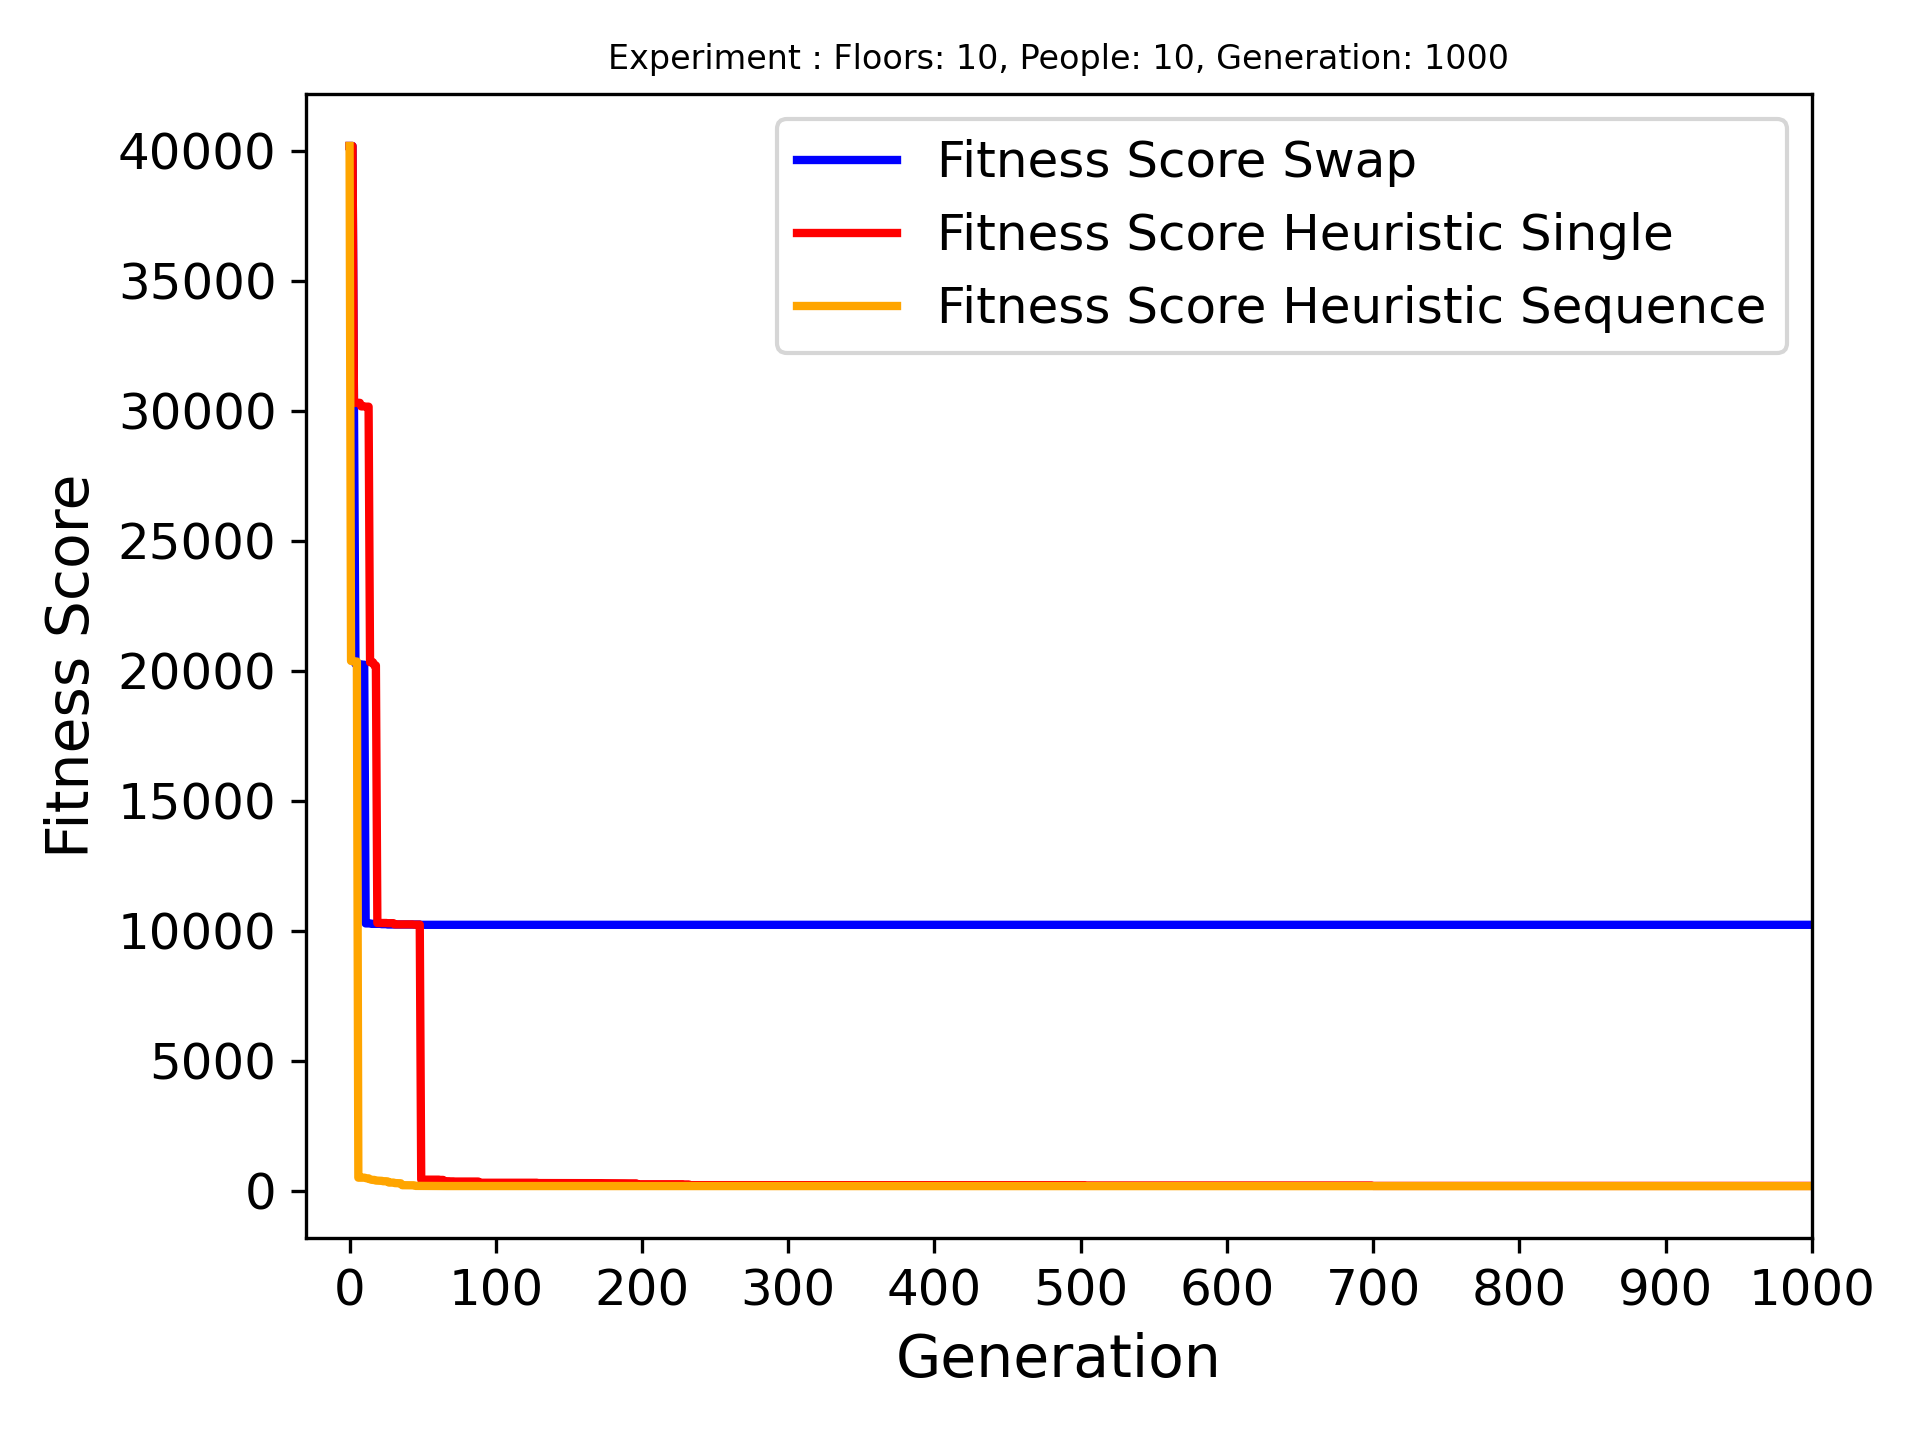
\includegraphics[width=\linewidth]{results/Building1/Mutation_0.1/Floors: 10, People: 10, Generation: 1000_worst.png}
		\captionsetup{justification=centering,font=tiny}
		\caption{Score/Arrived/Length:\\\textcolor{blue}{10227/9/9}, \textcolor{red}{182/10/11}, \textcolor{orange}{172/10/11}.}
		\label{fig:Building1/Mutation_0.1/Floors: 10, People: 10, Generation: 1000_worst}
	\end{subfigure}
	\hfill
	\begin{subfigure}[b]{0.49\linewidth}
		\centering
		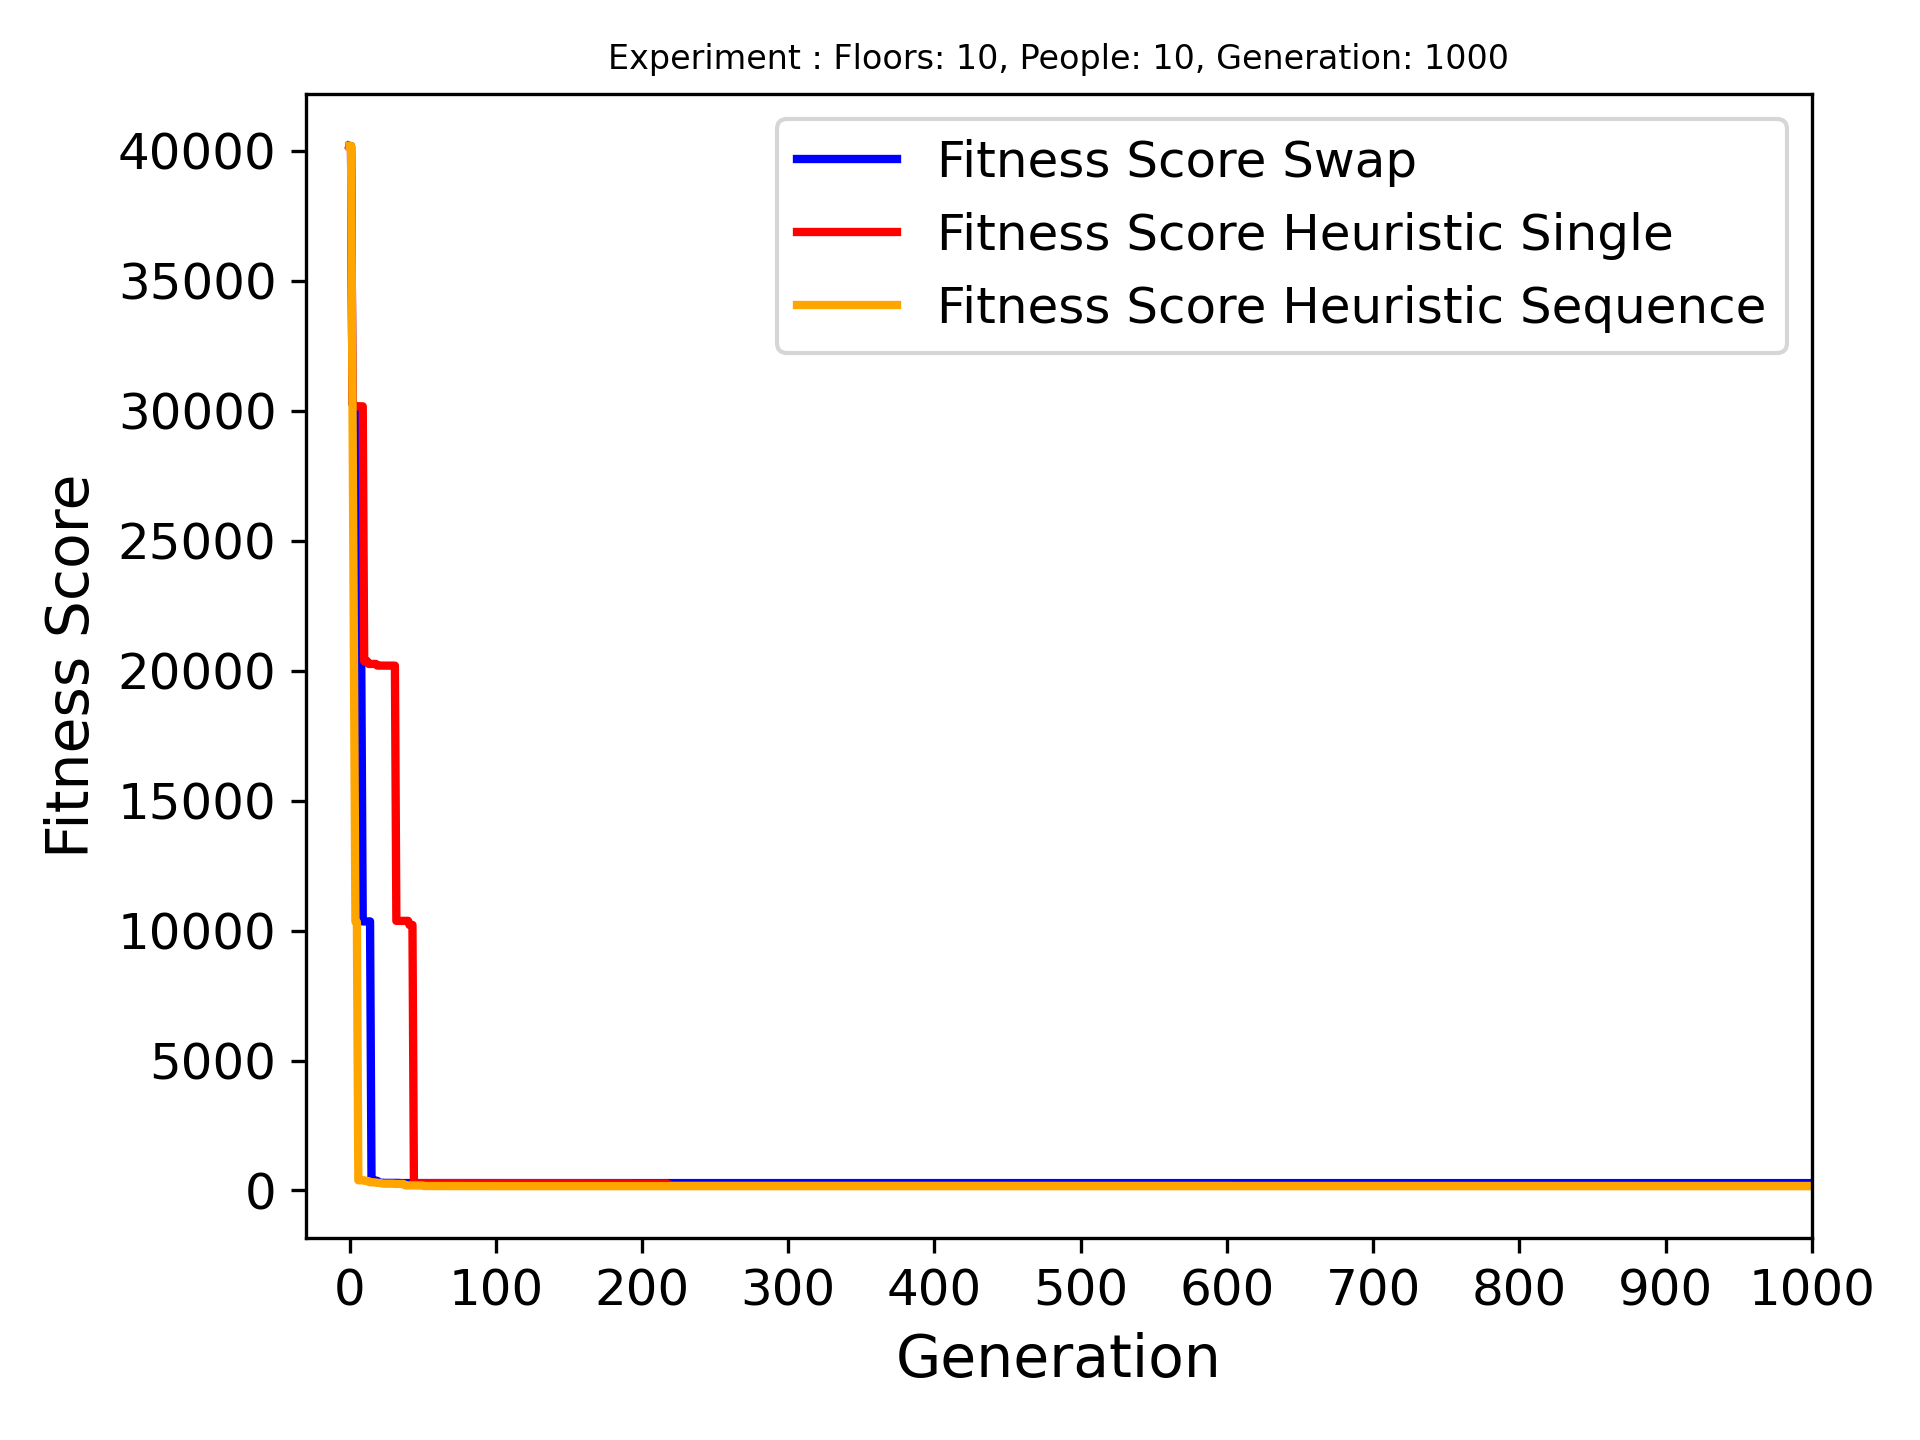
\includegraphics[width=\linewidth]{results/Building1/Mutation_0.1/Floors: 10, People: 10, Generation: 1000_best.png}
		\captionsetup{justification=centering,font=tiny}
		\caption{Score/Arrived/Length:\\\textcolor{blue}{284/10/11}, \textcolor{red}{187/10/14}, \textcolor{orange}{167/10/12}.}
		\label{fig:Building1/Mutation_0.1/Floors: 10, People: 10, Generation: 1000_best}
	\end{subfigure}
	\label{fig:Building 1 results}
	\captionsetup{font=scriptsize}
	\caption{Building 1 comparing worst and best case.}
\end{figure}
\subsection{Building 2}
Samuel had some papers he wanted to compare these results with.

\subsection{Building 3}
\begin{figure}[ht]
	\centering
	\begin{subfigure}[b]{0.49\linewidth}
		\centering
		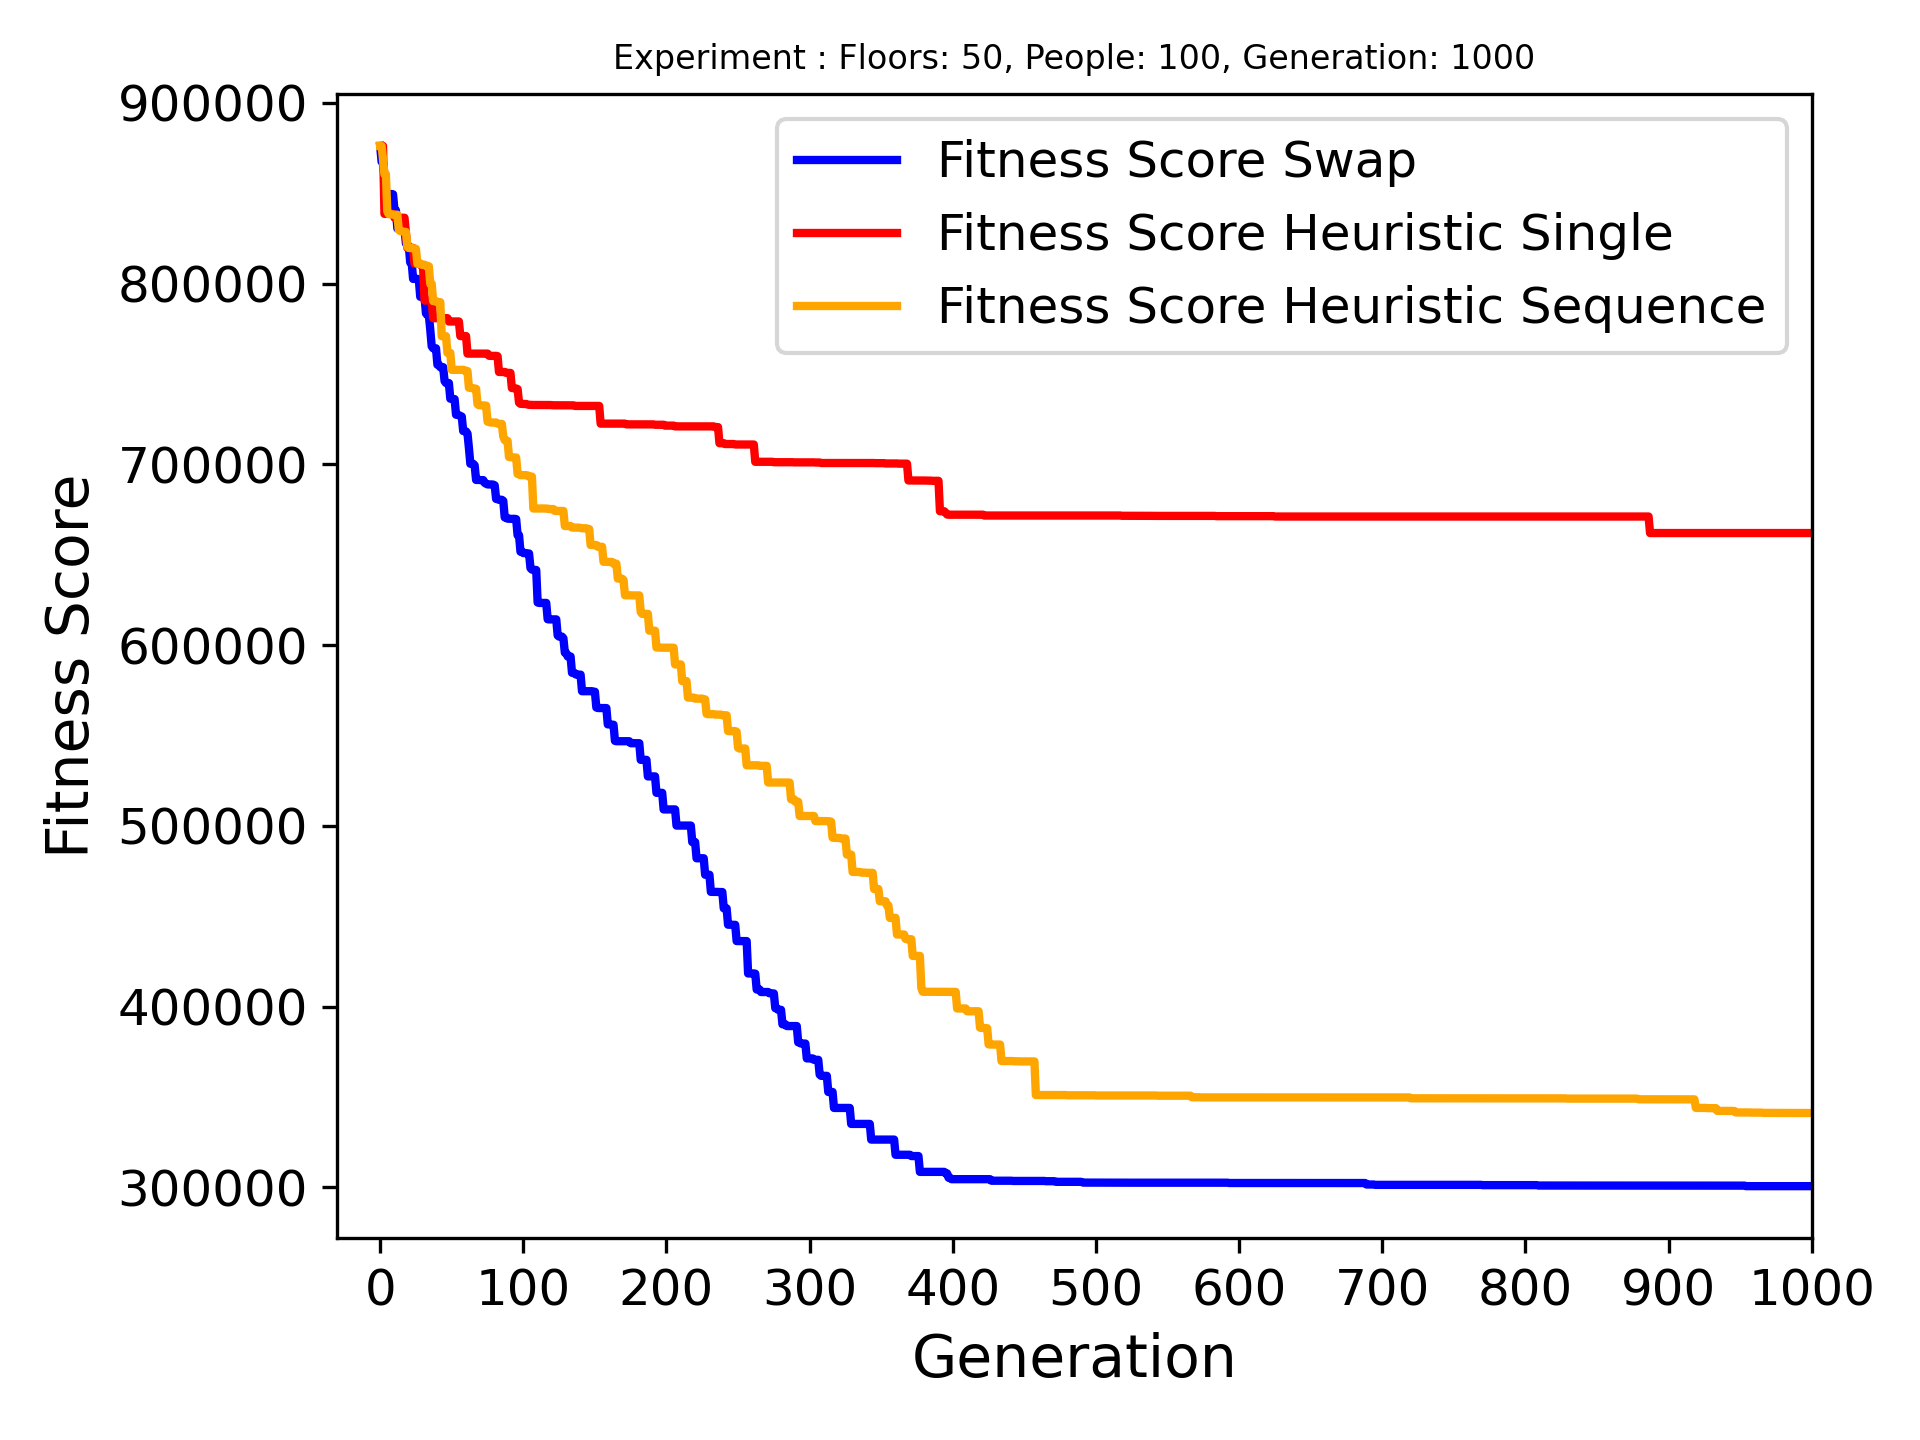
\includegraphics[width=\linewidth]{results/Building3/Mutation_0.1/Floors: 50, People: 100, Generation: 1000_4_worst.png}
		\captionsetup{justification=centering,font=tiny}
		\caption{Score/Arrived/Length:\\\textcolor{blue}{300697/74/69}, \textcolor{red}{661991/35/52}, \textcolor{orange}{341167/69/74}.}
		\label{fig:Building3/Mutation_0.1/Floors: 50, People: 100, Generation: 1000_4_worst}
	\end{subfigure}
	\hfill
	\begin{subfigure}[b]{0.49\linewidth}
		\centering
		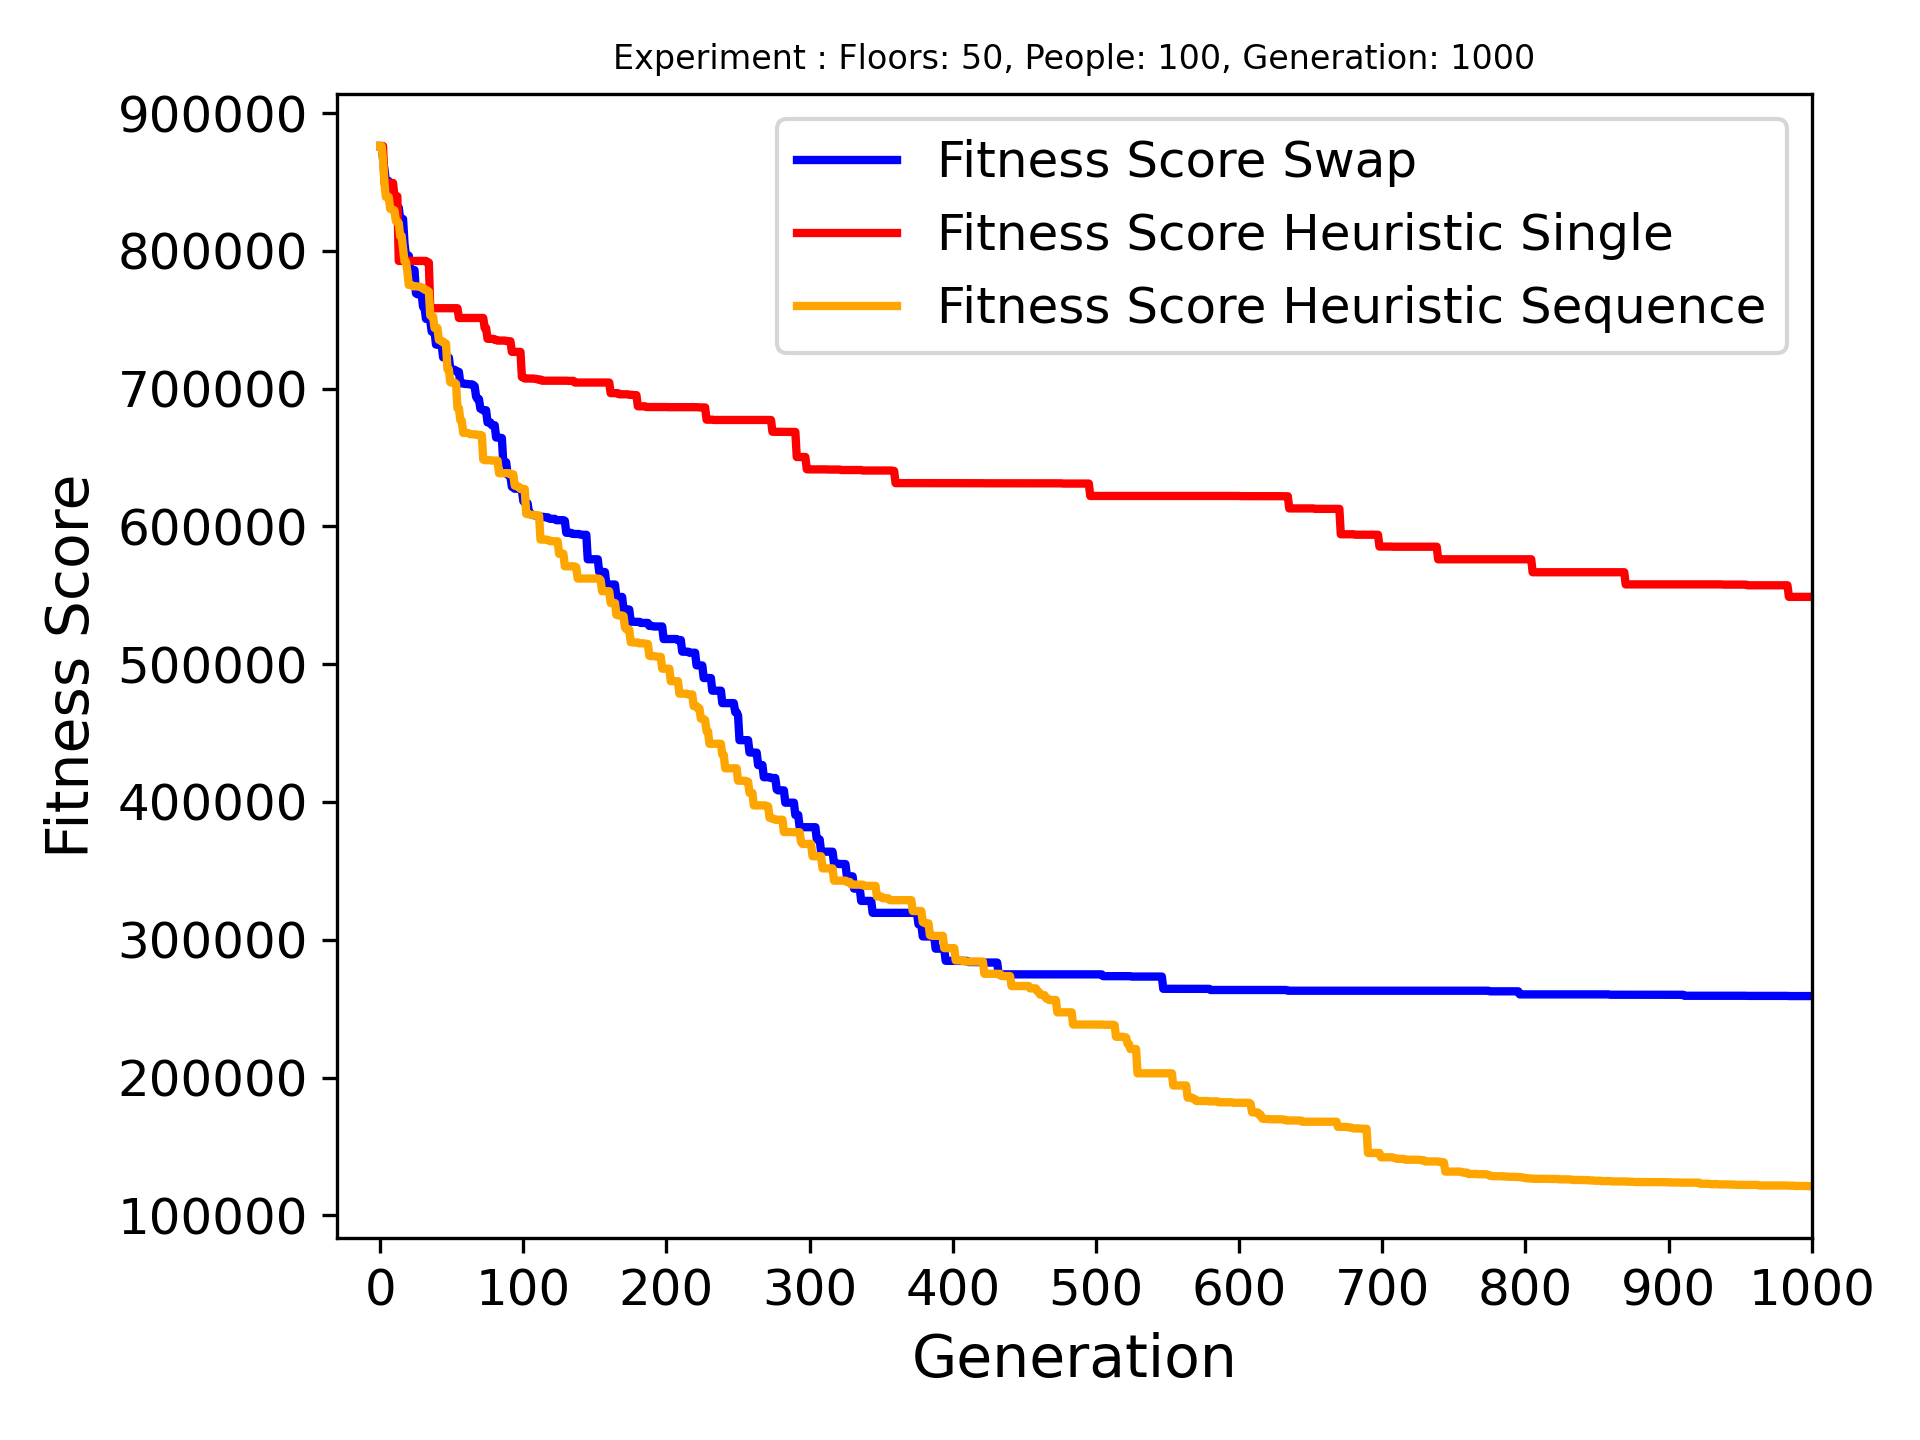
\includegraphics[width=\linewidth]{results/Building3/Mutation_0.1/Floors: 50, People: 100, Generation: 1000_1_best.png}
		\captionsetup{justification=centering,font=tiny}
		\caption{Score/Arrived/Length:\\\textcolor{blue}{259130/79/71}, \textcolor{red}{548857/48/59}, \textcolor{orange}{121157/94/124}.}
		\label{fig:Building3/Mutation_0.1/Floors: 50, People: 100, Generation: 1000_1_best}
	\end{subfigure}
	\captionsetup{font=scriptsize}
	\caption{Building 3 comparing worst and best case.}
	\label{fig:Building 3 comparing worst and best case}
\end{figure}

After running all the buildings with mutation rate of 0.1 we started testing out different values and quickly found out that our algorithm found a solution that serves all or almost all people much faster with a greater mutation rate. We ended up display result from runs with a mutation rate of 0.6. \ref{fig:Building 4 comparing different mutation rates} shows how much faster our algorithm reach acceptable solutions than before. When mutation rate was low the best solutions gave us a fitness scores around 500 000 but with a high rate we were able to get scores around 200 000. The best run served 66 people when mutation was 0.1, the best run with mutation 0.6 served all 100 people. Reason behind this is that to be able to serve as many people as possible the genes have to mutate to become longer or shorter. With a higher mutation rate this happens in much quicker pace and therefore the algorithm is able to leave local minimums faster. If we had more time to experiment with different mutation rates we could probably find an even better rate. In our situation mutation the genomes to become longer than the number of floors in the building is key to be able to serve all people. Therefore, a greater mutation rate is beneficial and less computational power is needed compared to increasing the population size or the number of generations. We tested increasing number of generations and received similar results as with a greater mutation rate.

\begin{figure}[ht]
	\centering
	\begin{subfigure}[b]{0.49\linewidth}
		\centering
		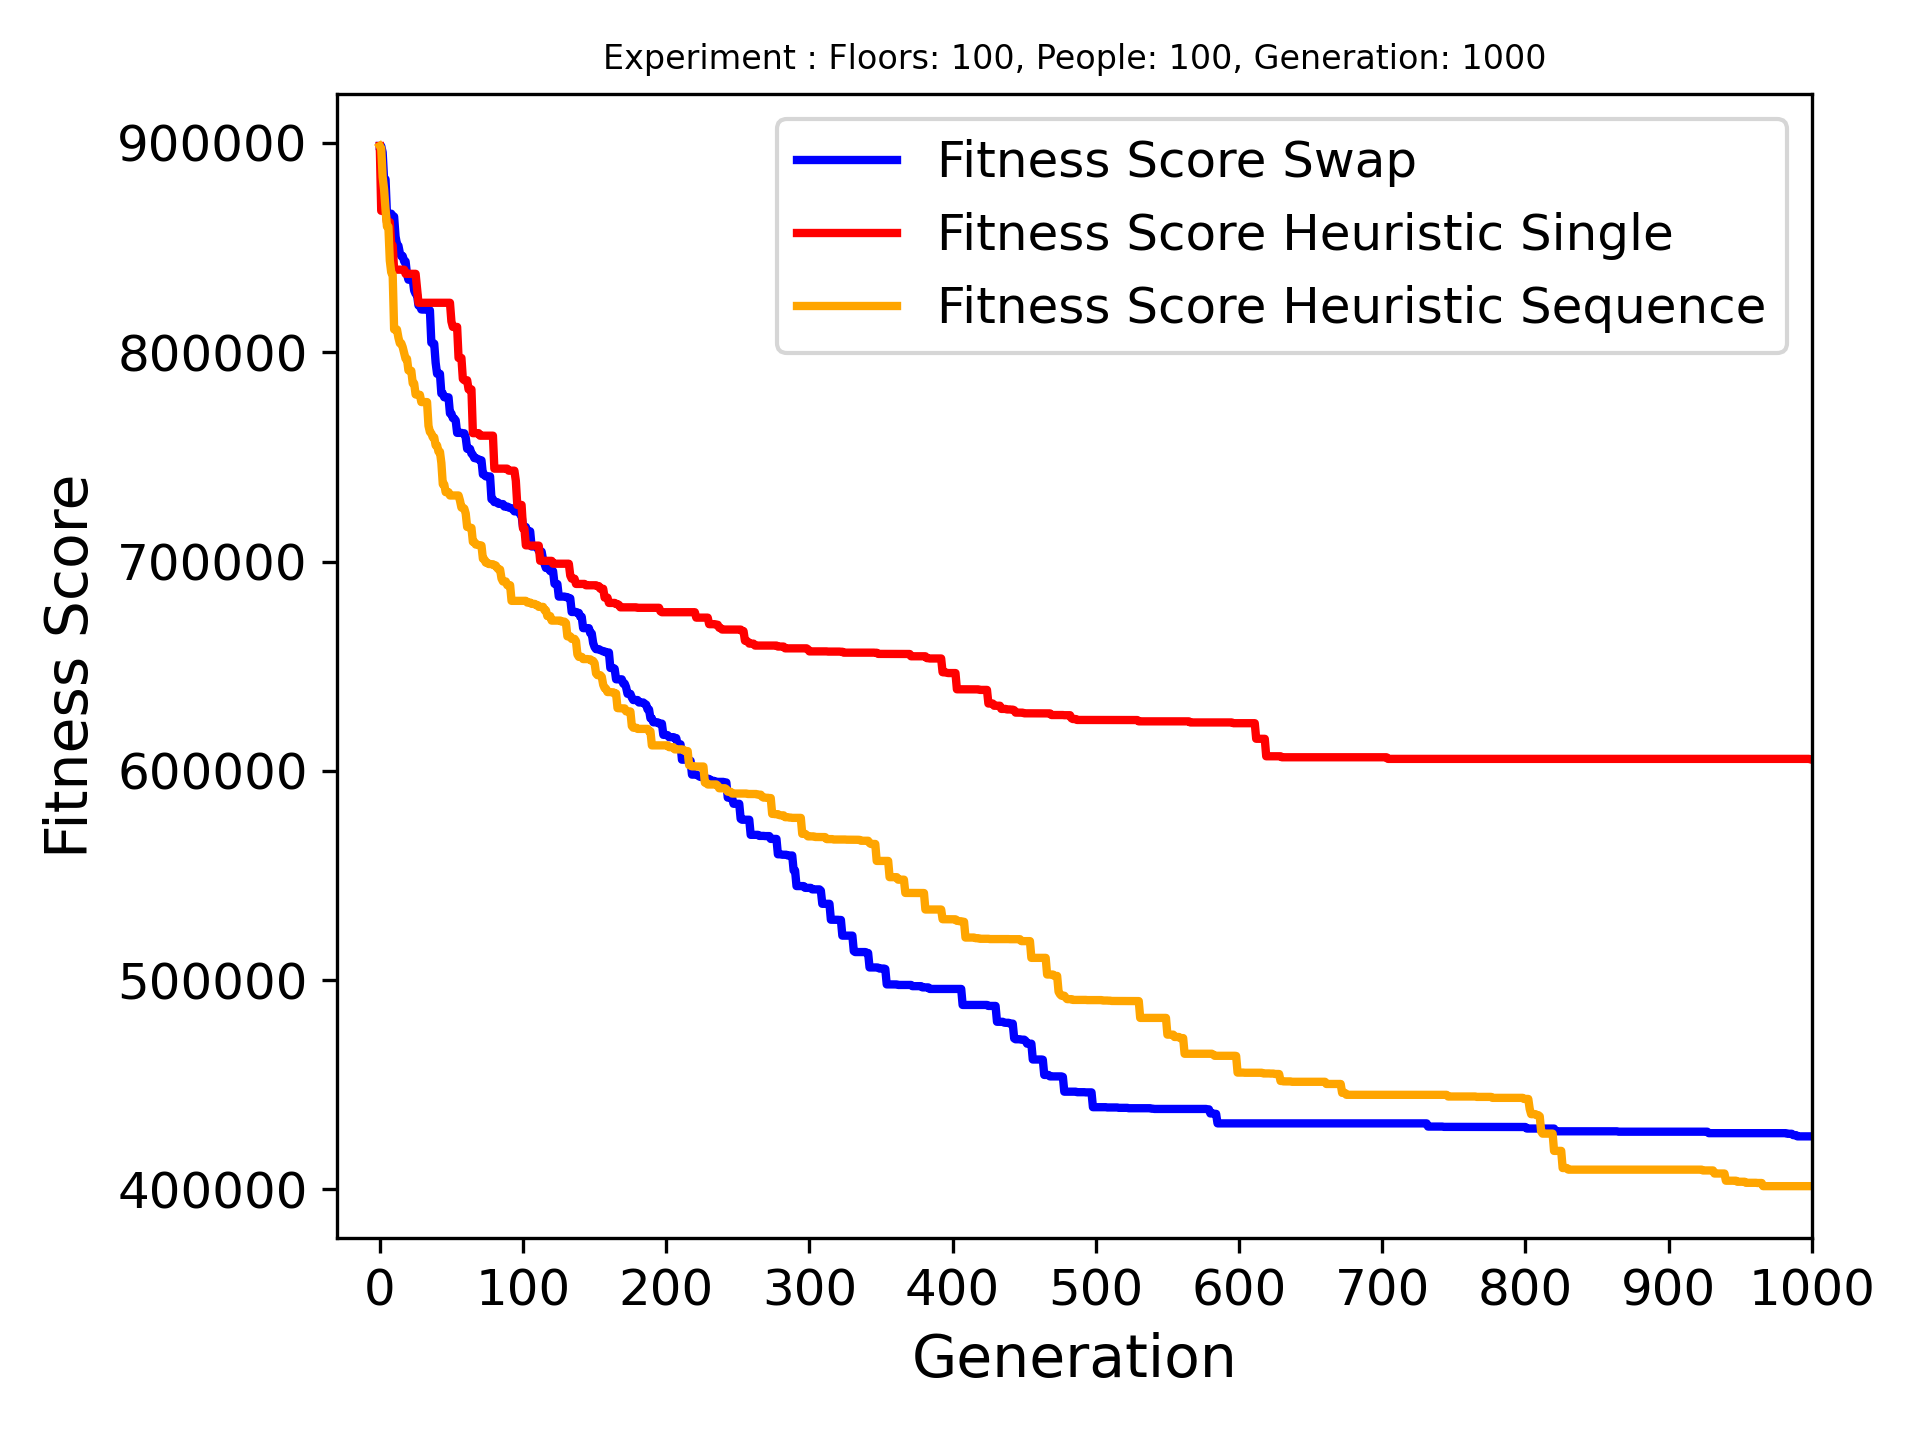
\includegraphics[width=\linewidth]{results/Building4/Mutation_0.1/Floors: 100, People: 100, Generation: 1000_2_best.png}
		\captionsetup{justification=centering,font=tiny}
		\caption{Score/Arrived/Length:\\\textcolor{blue}{425352/67/80}, \textcolor{red}{605508/44/102}, \textcolor{orange}{401562/66/75}.}
		\label{fig:Building4/Mutation_0.1/Floors: 100, People: 100, Generation: 1000_2_best}
	\end{subfigure}
	\hfill
	\begin{subfigure}[b]{0.49\linewidth}
		\centering
		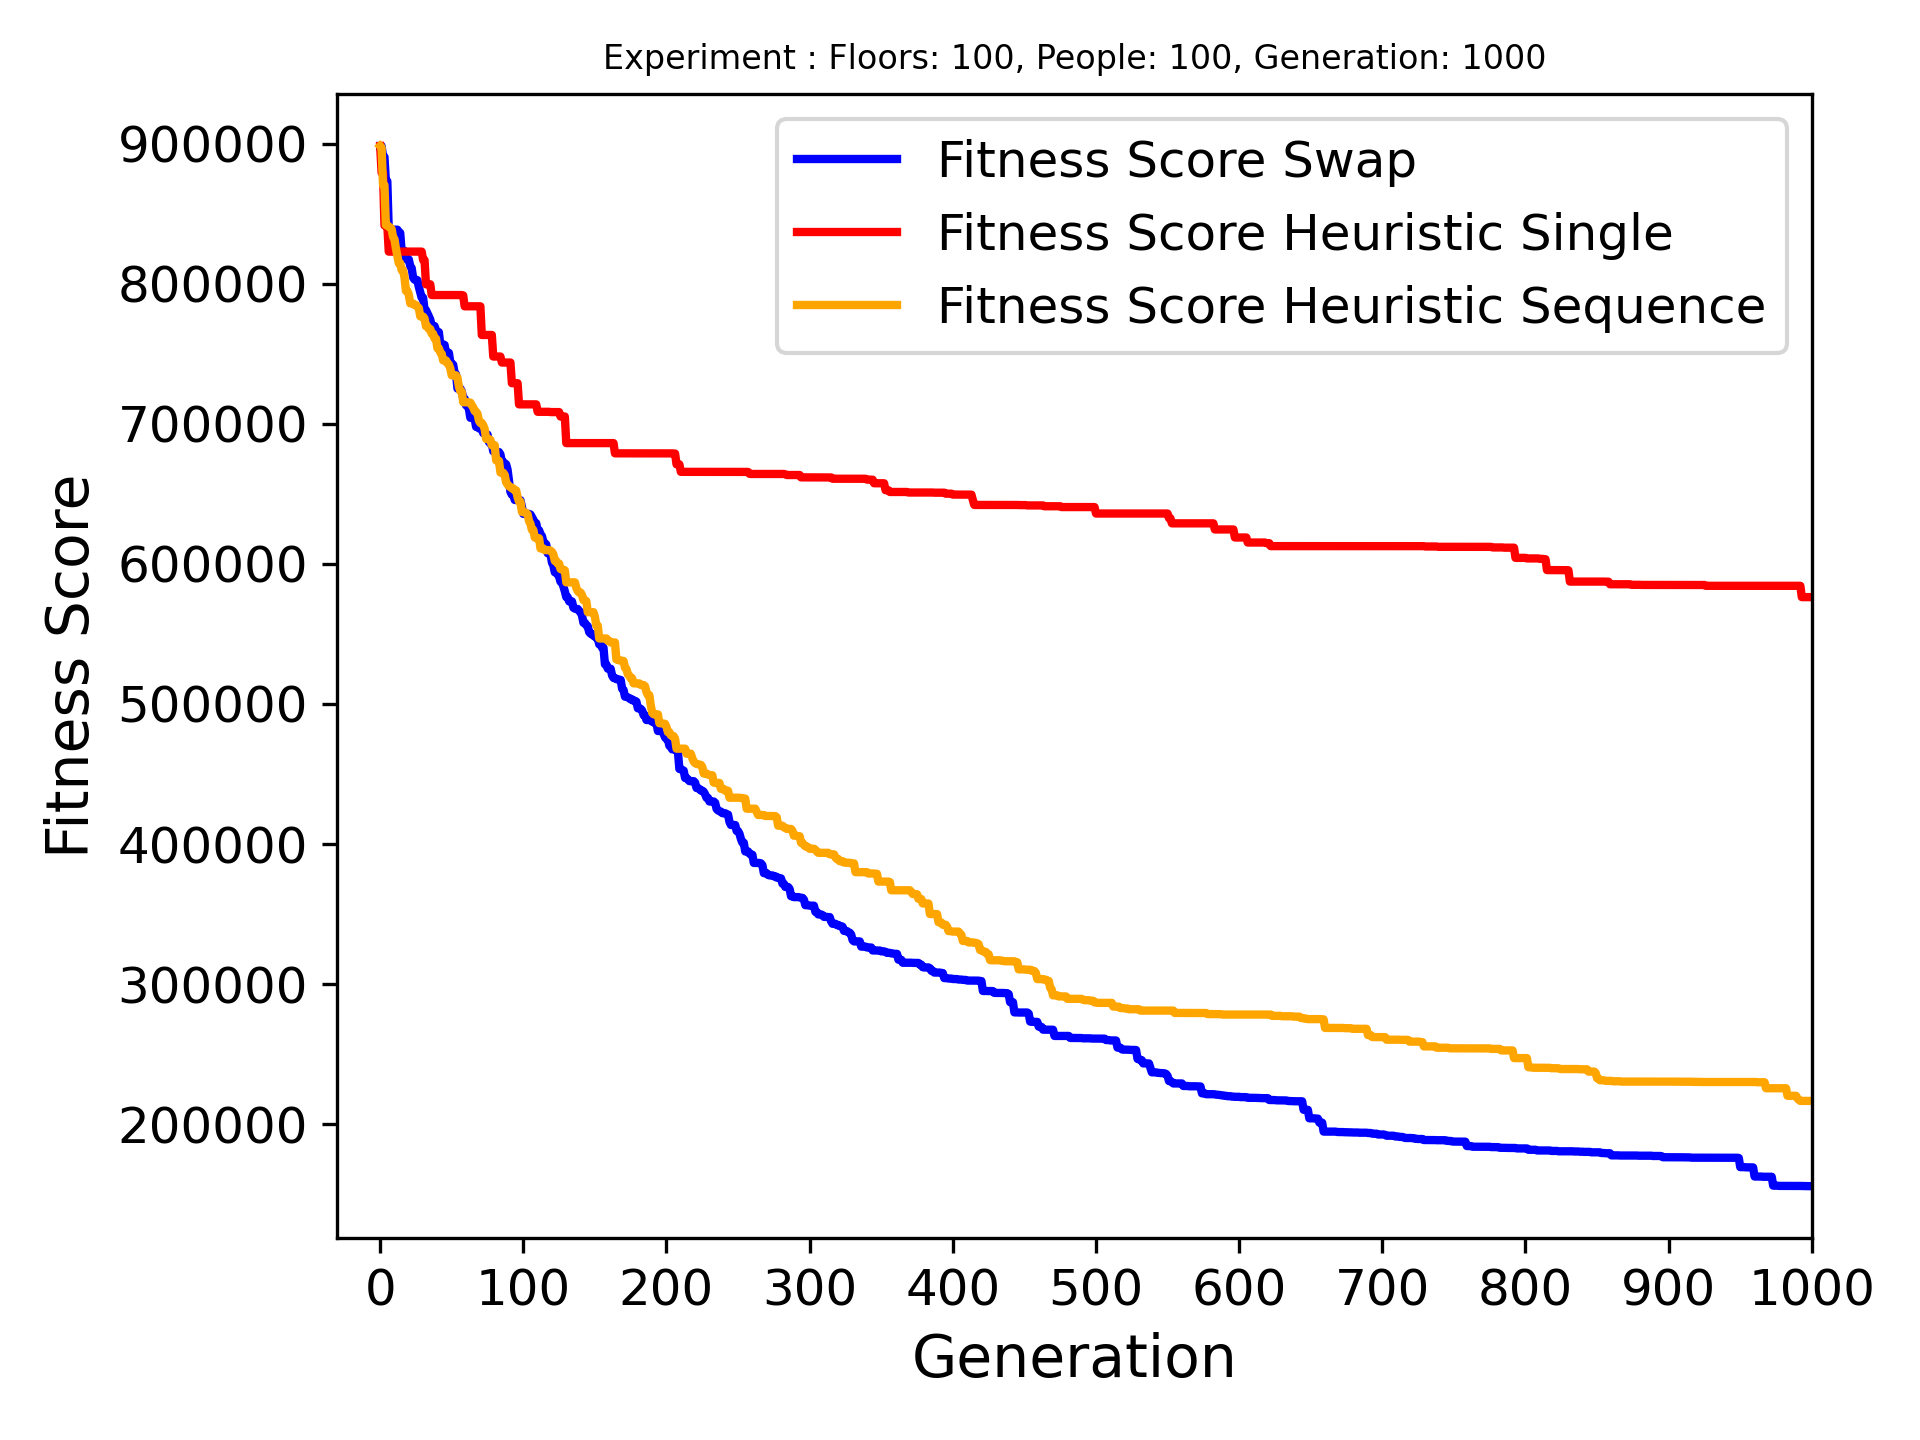
\includegraphics[width=\linewidth]{results/Building4/Mutation_0.6/Floors: 100, People: 100, Generation: 1000_best.png}
		\captionsetup{justification=centering,font=tiny}
		\caption{Score/Arrived/Length:\\\textcolor{blue}{155619/100/151}, \textcolor{red}{576322/48/117}, \textcolor{orange}{216508/94/139}.}
		\label{fig:Building4/Mutation_0.6/Floors: 100, People: 100, Generation: 1000_best}
	\end{subfigure}
	\captionsetup{font=scriptsize}
	\caption{Building 4 comparing different mutation rates.}
	\label{fig:Building 4 comparing different mutation rates}
\end{figure}


Thoughts:

— The first crossover can perform really well and even beet the third one in some cases, but it also tends to get stuck in local minima in some cases. This means that it is inconsistent and that you can't trust it to always give you a good solution. It performs worse with fewer people in the buildings.

— Too much diversity makes the second crossover bad, maybe it would have been better with more elitism and less diversity from mutations and roulette wheel selection. This crossover also have problems performing well on larger buildings with more people.

— The third crossover is the best one, due to that it always performs well and never gets stuck in local minima for long. This one performs well on all buildings and with all amounts of people. It also performs well with different mutation rates.
